\chapter{Implementacja serwisu}
\thispagestyle{chapterBeginStyle}

Rozdział ten zawiera dokumentację techniczną projektu. Zobrazowano sposób w jaki założenia projektowe, zostały zaimplementowane przy użyciu wybranych technologii. Zgodnie ze strukturą serwisu w podrozdziale pierwszym opisano sposób implementacji serwera, a podrozdziale drugim klienta. Przedstawiona ogólna dokumentacja miała na celu bliższe zapoznanie się ze sposobem działania serwisu pod względem informatycznym.

\section{Serwer}

Przy implementacji serwera wykorzystano głównie trzy moduły Firebase takie jak uwierzytelnianie, firestore (baza danych NoSQL) oraz funkcje. Komunikacja pomiędzy serwerem, a klientem opiera się na dwóch sposobach. Klient może bezpośrednio nasłuchiwać zmian zachodzących w bazie danych Firestore, albo wywoływać funkcje Firebase.

\subsection{Baza danych}

W bazie danych czasu rzeczywistego Firestore zostały umieszczone dwie kolekcje - \emph{Users}, \emph{Games}. W kolekcji \emph{Users} są przechowywane dokumenty indeksowane unikatowymi kodami ID użytkownika, które są przydzielane w czasie rejestracji. Każdy dokument zawiera pola \emph{name} i \emph{active}. Pole \emph{name} odnosi się do nazwy użytkownika, a pole \emph{active} jest wartością logiczną wskazującą, czy dany użytkownik jest dostępny w grze (jest zalogowany i obecnie nie znajduje się w rozgrywce z innymi graczami). Opcjonalne pole \emph{invitation} jest mapą zawierającą klucze \emph{gameId} oraz \emph{player}, których wartości wskazują kolejno na kod ID gry i nazwę gracza, który zaprosił danego gracza do swojej gry. W kolekcji \emph{Games} są przechowywane dokumenty indeksowane automatycznie generowanymi unikatowymi kodami ID przy tworzeniu dokumentu i które są przypisane jako kody ID gier. Każdy dokument zawiera trzy pola: \emph{available} (wskazuje ile graczy może jeszcze dołączyć do gry), \emph{currentTurn} (wskazuje jakiego gracza jest teraz kolej), \emph{size} (wskazuje na liczbę graczy w grze). Ponadto dokument danej gry zawiera jeszcze subkolekcje \emph{playersQueue}, \emph{playersRacks}, \emph{pool}, \emph{state}. \\ \\
Subkolekcja \emph{playersQueue} jest to zbiór dokumentów indeksowanych kodami ID graczy, którzy uczestniczą w tej grze. Każdy dokument zawiera pole \emph{name} z nazwą gracza oraz pole \emph{initialMeld}, które wskazuje czy dany gracz wyłożył już rozdanie początkowe. \\
Subkolekcja \emph{playersRack} to zbiór dokumentów z automatycznie generowanymi kodami ID. Dokumenty te przedstawiają kości, które są przydzielone graczowi. Każdy dokument zawiera dwa pola \emph{color} oraz \emph{number}. \\ \\
Subkolekcja \emph{pool} to z kolei zbiór dokumentów z automatycznie generowanymi kodami ID. Zbiór tych dokumentów przedstawia bank w grze, czyli wszystkie kości, które nie znajdują się na planszy ani nie są przydzielone do gracza. Każdy dokument ma pola \emph{color} oraz \emph{number}. \\ \\
Subkolekcja \emph{state} zawiera dokładnie jeden dokument \emph{sets} o najbardziej złożonej strukturze. W dokumencie \emph{sets} znajdują się wszystkie zbiory, które są wyłożone na planszy. Struktura tego dokumentu składa się z mapy, w której klucze to pozycja pierwszej kości z danego zbioru na planszy, a więc moment, w którym rozpoczyna się dany zbiór kości. Wartości tej mapy to tablica kości, gdzie każda kość jest w postaci mapy z kluczami \emph{color} i \emph{number}. Taki sposób przedstawienia stanu planszy wynika głównie z optymizacji kosztów modyfikowania bazy danych. Nie rozbito każdego zbioru kości na osobne dokumenty, ponieważ zwiększa to nam liczbę zliczanych zapisów do bazy danych. Ponadto w tym przypadku nie ma potrzeby korzystania z właściwości oferowanych przez dokumenty takie jak śledzenie zmian w danym dokumencie czy możliwość tworzenia prostych zapytań SQL na zbiorze dokumentów.

\subsection{Uwierzytelnianie}

Tak jak wspomniano wyżej występują dwa sposoby komunikacji klienta z serwerem. W przypadku funkcji Firebase do zapytań HTTPS z aplikacji, automatycznie są dołączane tokeny uwierzytelniania. W przypadku nasłuchiwaniu zmian zachodzących w bazie danych lub operacjach zaczytywania i modyfikowania bazy danych Firestore za proces autoryzacji dostępu są odpowiedzialne reguły bezpieczeństwa Firestore. \\ \\
W tym projekcie reguły bezpieczeństwa Firestore są zdefiniowane następująco:
\begin{itemize}
	\item w kolekcji \emph{users} użytkownik ma dostęp jedynie do dokumentu z własnym ID, na którym może wykonywać operacje czytania i modyfikacji,
	\item w kolekcji \emph{games} użytkownik ma dostęp jedynie do dokumentu gry, w którym on sam jest jednym z graczy. W tym dokumencie będzie miał dostęp do pól zdefiniowanych w dokumencie oraz do subkolekcji \emph{playersQueue} oraz \emph{playersRacks}. Co więcej w \emph{playersRacks} będzie miał dostęp jedynie do dokumentu z własnym polem ID. We wszystkich dostępnych miejscach użytkownik ma prawo jedynie wykonywać operacje czytania.
\end{itemize}

\subsection{Funkcje}

Za pomocą funkcji Firebase został zaimplementowany kod serwera serwisu. Jego głównymi zadaniami jest zarządzanie instancjami gier oraz uniemożliwienie prób oszukiwania w czasie rozgrywki przez graczy za pomocą ingerencji w kod źródłowy aplikacji po stronie klienta. \\ \\
Zbiór zdefiniowanych funkcji został uporządkowany w trzy podzbiory. W pierwszym podzbiorze znajdują się wszystkie możliwe do wywołania przez użytkownika funkcje serwera. Drugim podzbiorem jest klasa \emph{GameUtils}, zawierająca statyczne funkcje odpowiedzialne za zarządzanie instancjami gier. Trzecim podzbiorem jest klasa \emph{GameLogic}, zawierająca statyczne funkcje, które odpowiadają za walidację ruchów użytkowników w grze i implementację logiki rozgrywki gry. \\ \\
Charakterystyka funkcji serwera możliwych do wywołania przez użytkownika:
\begin{itemize}
	\item \emph{createGame} - jako paramtry wejściowe przyjmuje ID gracza i jego nazwę, listę nazw graczy zaproszonych do gry oraz czas przeznaczony na wykonanie ruchu w trakcie gry. \\
	Wywołuje ona metodę \emph{createGame} z klasy \emph{GameUtils}. Następnie wyszukuje poszczególnych graczy i informuje ich o zaproszeniu do gry. \\
	Parametrem zwracanym jest ID nowo utworzonej gry.
	\item \emph{searchGame} - jako parametry wejściowe przyjmuje ustawienia gry: liczbę graczy i czas przeznaczony na ruch gracza oraz ID gracza i jego nazwę. \\ 
	Wywołuje funkcję \emph{findGame} z \emph{GameUtils}. Jeśli gra zostanie znaleziona wywoływana jest funkcja \emph{addToGame}. Następnie jeśli gracz zajął ostatnie wolne miejsce w grze, wywoływana jest funkcja \emph{startGame} z \emph{GameUtils}. Jednak jeśli nie znaleziono gry, wywoływana jest funkcja \emph{createGame} z klasy \emph{GameUtils}.	Aby uchronić się przed wyszukiwaniem i modyfikowaniem bazy danych jednocześnie przez kilka wywołań funkcji \emph{searchGame} przez różnych graczy, proces wyszukania gry i zapisu do niej odbywa się poprzez transakcje. \\
	Parametrem wyjściowym jest ID gry.
	\item \emph{addToExistingGame} - jako parametry wejściowe przyjmuje ID gry oraz ID gracza i jego nazwę. \\
	Funkcja szuka instancji gry, a następnie wywołuje \emph{addToGame} z \emph{GameUtils}. Operacje na bazie danych również odbywają się z pomocą transakcji.
	\item \emph{putTiles} - jako parametry wejściowe przyjmuje ID gracza i gry oraz zbiór zbiorów kości znajdujących się na planszy. \\
	Znajduję instancję gry i subkolekcje graczy uczestniczących w niej, a następnie wywołuje metodę \emph{checkTurn} z \emph{GameLogic}. Potem nadaje prawo ruchu kolejnemu graczowi w kolejce. Dalej wywołuje metodę \emph{addNewTiles} z \emph{GameLogic}. Jeśli metoda ta zwróci, że gracz jest zwycięzcą, wskazuje zwycięzcę. Jeśli zwróci, że gracz nie wykonał żadnego ruchu lub próbował oszukiwać, to doda do jego zbioru kości kolejną kość z banku. W przypadku, gdy była to ostatnia kość z banku, to wywołuje metodę \emph{pointTheWinner} z \emph{GameLogic}.
	\item \emph{leftGame} - jako parametry wejściowe przyjmuje ID gracza i gry. \\
	Usuwa gracza z kolejki graczy w grze. Jeśli akurat ten gracz miał prawo ruchu, daje możliwość ruchu następnemu graczowi. \\
\end{itemize}
Charakterystyka funkcji statycznych serwera z klasy \emph{GameUtils}:
\begin{itemize}
	\item \emph{createGame} - tworzy dokument gry w kolekcji \emph{games}. Dodaje założyciela do subkolekcji \emph{playersQueue} oraz tworzy wszystkie możliwe kości w postaci dokumentów i dodaje je do subkolekcji \emph{pool}. \\
	Zwraca ID gry.
	\item \emph{addToGame} - dodaje gracza do istniejącej już gry. \\
	Zwraca ID gry oraz wartość logiczną dotyczącą występowania wolnych miejsc w grze.
	\item \emph{findGame} -  za pomocą parametrów ustawień gry (liczba graczy, czas na ruch) szuka wolnej instancji gry. \\
	Zwraca instancję gry lub null.
	\item \emph{startGame} -  przydziela graczom po 14 kości losowo wybranych z subkolekcji \emph{pool}. Nadaje prawo do wykonania ruchu pierwszego graczowi w subkolekcji \emph{playersQueue}. \\ 
\end{itemize}
Charakterystyka funkcji statycznych serwera z klasy \emph{GameLogic}:
\begin{itemize}
	\item \emph{checkTurn} - sprawdza, czy dany gracz ma prawo wyłożyć kości.
	\item \emph{addNewTiles} - przeprowadza walidację nowego zbioru kości na planszy. Sprawdza, czy zbiory są poprawnie ułożone, czy występują wszystkie poprzednie kości na planszy, czy nowo położone kości należą do gracza. W przypadku wyłożenia początkowego sprawdza czy gracz wyłożył nowe ułożenia o wartości co najmniej 30 punktów oraz czy poprzednie ułożenie nie zostały zmodyfikowane. Po spełnieniu tych warunków usuwa nowo wyłożone kości z puli gracza i modyfikuje stan planszy. W przypadku wyłożenia początkowego odznacza, że zostało wykonane. \\
	Zwraca informację, czy kości zostały poprawnie dodane lub informację, że gracz zwyciężył w przypadku usunięcia wszystkich kości z jego puli.
	\item \emph{getTileFromPool} - wybiera jedną kość z subkolekcji \emph{pool} i przydziela je danemu graczowi. \\
	Zwraca informację, czy w \emph{pool} znajdują się jeszcze dostępne kości.
	\item \emph{pointTheWinner} -  sumuje wszystkie wartości kości w poszczególnych pulach graczy. Wskazuje zwycięzcę lub zwycięzców w przypadku równości sum.
\end{itemize}

\section{Klient}

Warstwa klienta w serwisie napisana we Flutterze jest dostępna jako aplikacja na telefon albo jako strona internetowa. Z uwagi na wieloplatformowość Fluttera kod źródłowy obu wersji klienta jest wspólny z odpowiednimi konfiguracjami i modyfikacjami na poszczególne platformy.

\subsection{Warstwa prezentacji}

W warstwie prezentacji zdefiniowany jest wygląd aplikacji klienta. Warstwa ta składa się z bezstanowych widgetów, które generują interfejs graficzny. Klasy te odpowiadają za odbieranie
komunikatów ze strony użytkownika jak i przekazują lub odbierają komunikaty ze strony logiki aplikacji. Zdarzenia te mogą mieć wpływ na wygląd danego widgeta. Komunikacja pomiędzy poszczególnymi stronami aplikacji jest również zdefiniowana w tej warstwie. \\

Nawigacja pomiędzy stronami odbywa się poprzez dynamiczną nawigacją z wygenerowanymi trasami. Jest to jeden ze sposobów komunikacji we Flutterze, dzięki któremu za cały proces nawigacji odpowiada klasa \emph{app\_router}, a w poszczególnych widgetach podaje się nazwę ścieżki i obiekty do przekazania pomiędzy stronami. Główną zaletą korzystania z tego sposobu jest eliminacja bezpośrednich zależności pomiędzy widgetami. Ponadto zmniejsza się objętość kodu, a sam kod staje się bardziej przejrzysty. \\

\begin{figure}[h!]
	\begin{center}
		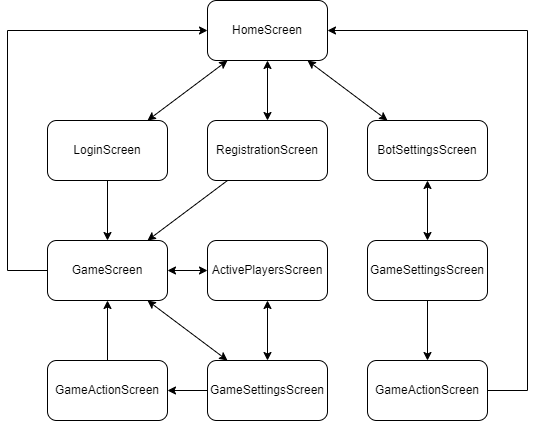
\includegraphics[width=13cm,height=10cm]{img/nawigacja.png}
	\end{center}
	\caption{{\color{dgray}Diagram nawigacji.}} 
	\label{nawigacja}
\end{figure}  

\emph{HomeScreen} jest ekranem startowym aplikacji, od którego zaczyna się każda inna ścieżka. W programie można podążyć dwoma głównymi ścieżkami. Pierwszą ścieżką jest wybranie gry z botem lokalnie na urządzeniu użytkownika bez konieczności połączenia z internetem. Następnie wybraniu ustawień bota i kolejno ustawień gry i przejściu do rozgrywki. Po wyjściu z gry użytkownik wraca do ekranu startowego. Drugą ścieżką jest z kolei zalogowanie się lub utworzenie konta gracza. Następnie użytkownik będzie miał do wyboru sposób rozpoczęcia gry. Jeśli zdecyduje się na utworzenie własnej gry z innymi aktywnymi użytkownikami, przechodzi do strony \emph{ActivePlayersScreen}, a dalej do ustawień gry. Jeśli jednak będzie chciał dołączyć do istniejącej już gry, aplikacja przekierowuje go bezpośrednio do \emph{GameSettingsScreen}. Po przejściu do rozgrywki gracz w każdej chili może opuścić grę. W takim przypadku znajdzie się z powrotem w \emph{GameScreen}. Z którego również może nastąpić wylogowanie się użytkownika i powrót do ekranu startowego. \\ \\ 
Charakterystyka poszczególnych klas w warstwie prezentacji:
\begin{itemize}
	\item \emph{AppRouter} - klasa odpowiadająca za nawigację w aplikacji. Zawiera zdefiniowane ścieżki, które wskazują na poszczególne strony. Jest odpowiedzialna za tworzenie nowego ekranu i dołączanie do niego odpowiednich zależności i przekazywanych parametrów.
	\item \emph{HomeScreen} - klasa zawierająca trzy przyciski kolejno prowadzące do \emph{RegirstrationScreen}, \emph{LoginScreen}, \emph{BotSettingsScreen}. Ekran startowy aplikacji.s
	\item \emph{RegirstrationScreen} - klasa zawierająca formularz z danymi do rejestracji (email, nazwa gracza, hasło, potwierdzenie hasła). Przeprowadza walidację formatu email oraz długości hasła i jego identyczności z potwierdzającym hasłem.
	\item \emph{LoginScreen} - klasa zawierająca formularz z potrzebnymi danymi do zalogowania użytkownika (email, hasło).
	\item \emph{BotSettingsScreen} - klasa zawierająca dwa przyciski, odpowiadające za wybrany poziom bota. Przekierowują one do ekranu \emph{GameSettings} z argumentami \emph{playerId} oraz \emph{serverType}, co w przypadku gry z botem będzie równoznacze z numerem ID gracza \emph{0} oraz typ serwera \emph{basicBot}, \emph{advancedBot}.
	\item \emph{GameScreen} - klasa zawierająca dwa przyciski, które definiują sposób dołączenia do rozgrywki. Prowadzą one do stron \emph{ActivePlayersScreen}, \emph{GameSettingsScreen} i jako parametr przekazują ID gracza. Ponadto, gdy użytkownik chce powrócić do wcześniejszej strony zostanie wyświetlone okno dialogowe, wymuszające potwierdzenie decyzji, gdyż wiążę się ona z wylogowaniem użytkownika i powrotem do ekranu startowego. W przypadku, gdy użytkownik zostanie zaproszony do gry przez innego gracza, również zostanie wyświetlone okno dialogowe, w którym gracz będzie mógł przyjąć lub odrzucić zaproszenie.
	\item \emph{ActivePlayersScreen} - składa się z wyszukiwarki, listy aktywnych użytkowników oraz przycisku. Lista aktywnych użytkowników jest sortowana względem wyrazu wpisanego do wyszukiwarki. Użytkownik wybiera z listy graczy, których chce zaprosić do gry. Po kliknięciu w przycisk przechodzi do \emph{GameSettings} z parametrami \emph{playerId} (ID użytkownika), \emph{selectedPlayers} wybrani gracze, \emph{serverType} (nazwę serwera).
	\item \emph{GameSettingsScreen} - klasa zawierająca dwa pola przeznaczone do konfiguracji liczby uczestników i czasu przeznaczonego na ruch gracza oraz przycisk. Po kliknięciu w przycisk ukazuje się obracające kółeczko i napis z liczbą graczy brakujących do rozpoczęcia rozgrywki. Po pojawieniu się wymaganej liczby graczy nastąpi przekierowanie do \emph{GameActionScreen} z parametrami \emph{gameId}, \emph{playerId}, \emph{serverType}.
	\item \emph{GameActionScreen} - klasa obrazująca całą rozgrywkę w grę Rummikub. W górnej części znajduję się panel, na którym widać wszystkich uczestników i ilość pozostałego czasu dla aktualnie grającego gracza oraz przycisk zatwierdzający ruch. W środkowej części znajduje się plansza, na której można umieszczać swoje kości tworząc lub rozbudowując obecnie znajdujące się tam kości. W dolnej części umieszczony jest zbiór kości, które aktualnie posiada gracz. Komunikaty informacyjne o występujących zdarzeniach w czasie rozgrywki są pokazywane w postaci znikających dymków (toasty).
\end{itemize}

\subsection{Warstwa logiki}

W warstwie logiki zdefiniowane są zasady działania aplikacji. Z racji wykorzystanego wzorca projektowego we Flutterze klasy te są w postaci cubitów. Instancje tych klas są tworzone w klasie \emph{AppRouter} i odpowiednio są powiązane z klasami w warstwie prezentacji. Do każdego cubita przypisany jest zbiór klas, które reprezentują poszczególne stany. Klasy stanowe są przekazywane za pomocą strumienia do odpowiednich klas w warstwie prezentacji. \\ \\
Charakterystyka poszczególnych cubitów:
\begin{itemize}
	\item \emph{AuthCubit} - klasa ta jest powiązana z czynnościami dotyczącymi bezpośrednio konta użytkownika. Przeprowadza rejestrację, logowanie i wylogowanie gracza. Ponadto powiadamia użytkownika, gdy ten zostanie zaproszony do gry przez innego gracza i w przypadku akceptacji dołącza go do gry.
	\item \emph{GameSettingsCubit} - klasa odpowiadająca za konfigurację gry. Zawiera stan zawierający wybrane ustawienia gry. Odpowiada również za proces dołączania do gry (wyszukanie gry lub jej stworzenie oraz oczekiwanie na pozostałych graczy).
	\item \emph{ActivePlayersCubit} - klasa pobiera aktywnych użytkowników i odpowiednio je filtruje na podstawie podanej przez użytkownika wartości. Zawiera stan wskazujący na obecnie wybranych graczy.
	\item \emph{GameActionPanelCubit} - klasa zarządzająca rozgrywką. Przechowuje stan, który zawiera listę uczestników oraz pozostały czas na ruch obecnie grającego. Zarządza kolejką graczy, jak również informuje o wyniku końcowym gry. Ponadto umożliwia użytkownikowi opuszczenie rozgrywki przed zakończeniem.
	\item \emph{GameActionBoardCubit} - klasa odpowiadająca za planszę gry. Stan klasy zawiera listę obecnie ułożonych zestawów kości na planszy. Cubit ten odpowiada za aktualizowanie planszy w przypadku wyłożeń gracza lub innych graczy. W przypadku wyłożeń użytkownika przeprowadza walidację oraz zgodność z regułami gry i odpowiednio modyfikuje stan planszy.
	\item \emph{GameActionRackCubit} - klasa zawierająca stan, który przechowuje kości użytkownika. Jest odpowiedzialna za modyfikację tego stanu w przypadku wyłożeń użytkownika lub gdy użytkownik dostaje kość z banku.
\end{itemize}

\subsection{Warstwa danych}

Warstwa danych składa się z dwóch interfejsów \emph{AuthRepository} oraz \emph{GameRepository}. Pierwszy interfejs odpowiada za zarządzanie kontem użytkownika, a drugi instancją gry. W aplikacji obecnie zaimplementowane są dwa rozwiązania będące warstwą danych: firebase, bot. \\ \\
Charakterystyka interfejsu \emph{AuthRepository}:

\begin{itemize}
	\item \emph{signUp} - metoda asynchroniczna, która jako parametry wejściowe przyjmuje email, nazwę oraz hasło użytkownika. Odpowiada za zarejestrowanie się do serwisu. Zwraca klasę \emph{Player}, która zawiera nazwę i ID gracza.
	\item \emph{logIn} - metoda asynchroniczna, która jako parametry wejściowe przyjmuje email oraz hasło użytkownika. Odpowiada za zalogowanie się do serwisu. Zwraca klasę \emph{Player}, która zawiera nazwę i ID gracza.
	\item \emph{logOut} - metoda asynchroniczna, która jako parametry wejściowe przyjmuje ID gracza. Odpowiada za wylogowanie się z serwisu.
	\item \emph{invitationToGame} - metoda, która jako parametry wejściowe przyjmuje ID użytkownika. Zwraca strumień, przez którego będą wysyłane zaproszenia do gry.
	\item \emph{activePlayers} - metoda, która jako parametry wejściowe przyjmuje ID użytkownika. Zwraca strumień, przez którego będą wysyłani obecnie aktywni gracze. \\
\end{itemize}
Charakterystyka interfejsu \emph{GameRepository}:

\begin{itemize}
	\item \emph{createGame} - metoda asynchroniczna, która jako parametry wejściowe przyjmuje ID gracza, listę nazw zaproszonych graczy oraz czas przeznaczony na ruch w grze. Jest wywoływana w momencie, gry gracz tworzy własną grę i zaprasza innych graczy. Zwraca ID nowo utworzonej gry.
	\item \emph{searchGame} - metoda asynchroniczna, która jako parametry wejściowe przyjmuje ID gracza, liczbę graczy w grze oraz czas przeznaczony na ruch w grze. Jest wywoływana w momencie, gdy gracz chce znaleźć grę o podanych parametrach. Zwraca ID znalezionej gry lub w przypadku jej braku zwraca ID nowo utworzonej gry.
	\item \emph{joinGame} - metoda asynchroniczna, która jako parametry wejściowe przyjmuje wartość logiczną wskazującą na dołączenie do rozgrywki oraz ID gry. Jest wywoływana w momencie, gry gracz otrzymał zaproszenie do gry.
	\item \emph{missingPlayers} - metoda, która jako parametry wejściowe przyjmuje ID gry. Zwraca strumień, przez którego będzie wysyłana liczba brakujących graczy do rozpoczęcia rozgrywki.
	\item \emph{playerTiles} - metoda, która jako parametry wejściowe przyjmuje ID użytkownika oraz ID gry. Zwraca strumień, przez którego będą wysyłane kości należące do gracza.
	\item \emph{playersQueue} - metoda, która jako parametry wejściowe przyjmuje ID gry. Zwraca strumień, przez którego będą wysyłani gracze uczestniczący w grze.
	\item \emph{gameStatus} - metoda, która jako parametry wejściowe przyjmuje ID gry. Zwraca strumień, przez którego będzie wysyłany aktualny stan gry, czyli gracz mający ruch, czas przeznaczony na ruch oraz zwycięzca gry.
	\item \emph{tilesSets} - metoda, która jako parametry wejściowe przyjmuje ID gry. Zwraca strumień, przez którego będą wysyłane zbiory kości znajdujące się na planszy.
	\item \emph{putTiles} - metoda asynchroniczna, która jako parametry wejściowe przyjmuje ID gry oraz zbiory kości znajdujące się na planszy. Odpowiada za przekazanie wykonanego ruchu gracza.
	\item \emph{leaveGame} - metoda asynchroniczna, która jako parametry wejściowe przyjmuje ID gry, ID użytkownika. Obsługuje wyjście gracza z rozgrywki.	\\
\end{itemize}
W przypadku firebase zdefiniowane są dwie klasy \emph{AuthFirebase} oraz \emph{GameFirebase}, które implementują odpowiednie interfejsy. Klasy te są odpowiedzialne za komunikację z platformą Firebase. \\

\begin{figure}[h!]
	\begin{center}
		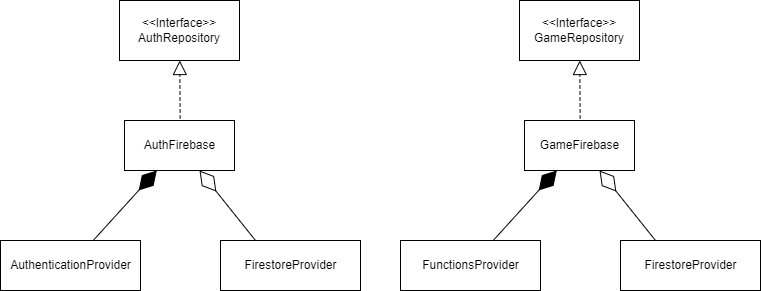
\includegraphics[width=16cm,height=6cm]{img/firebase-client.png}
	\end{center}
	\caption{{\color{dgray}Diagram klas warstwy danych firebase.}} 
	\label{firebase}
\end{figure}  

Klasa \emph{AuthFirebase} jest w relacji z klasą \emph{AuthenticationProvider} w postaci agregacji całkowitej (kompozycji). Oznacza to, że klasa główna (\emph{AuthFirebase}) ma na własność klasę częściową (\emph{AuthenticationProvider}) i kontroluje cykl życia części. Natomiast pomiędzy \emph{AuthFirebase}, a \emph{FirestoreProvider} występuje relacja agregacji częściowej. To znaczy, że element częściowy (\emph{FirestoreProvider}) należy do elementu głównego (\emph{AuthFirebase}), ale nie jest od niego zależny. Usunięcie elementu głównego, nie wpłynie na element częściowy. W przypadku \emph{GameFirebase} występuje ona w relacji częściowej z \emph{FirestoreProvider}, a w relacji agregacji całkowitej z \emph{FirestoreProvider}. Zatem z klasy \emph{FirestoreProvider} korzysta się w obu klasach implementujących interfejsy warstwy danych. 

Klasa \emph{AuthenticationProvider} odpowiada za połączenie się z usługą \emph{Firebase Authentication} i przeprowadzanie operacji zarejestrowania, zalogowania i wylogowania użytkownika. 

Klasa \emph{FirestoreProvider} odpowiada za połączenie się z usługą \emph{Firebase Firestore} (baza danych czasu rzeczywistnego). Klasa ta czyta lub zapisuje dane do bazy danych. Ponadto tworzy strumienie, które nasłuchują zmiany zachodzące w wybranych miejscach w bazie danych. 

Klasa \emph{FunctionsProvider} odpowiada za połączenie się z usługą \emph{Firebase Functions}. Wywołuje dedykowane funkcje po stronie serwera. 
W przypadku bota zdefiniowana jest jedna klasa \emph{GameBot}, która implementuje interfejs \emph{GameRepository}. Klasa ta zarządza instancją gry, która jest tworzona lokalnie na urządzeniu użytkownika. Biorąc pod uwagę rozwiązanie w postaci bota, konto użytkownika nie jest w użyciu. 

\begin{figure}[h!]
	\begin{center}
		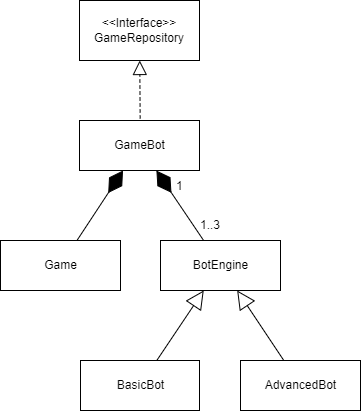
\includegraphics[width=8cm,height=9cm]{img/bot-client.png}
	\end{center}
	\caption{{\color{dgray}Diagram klas warstwy danych bot.}} 
	\label{bot}
\end{figure}

Klasa \emph{GameBot} występuje w relacji agregacji całkowitej z klasami \emph{Game} oraz \emph{BotEngine}. Klasa główna może zawierać od 1 do 3 instancji klasy \emph{BotEngine}. To ograniczenie wzięło się z zasady, że w grę Rummikub może grać od 2 do 4 graczy. Klasy \emph{BasicBot} i \emph{AdvancedBot} dziedziczą po klasie \emph{BotEngine}. 

Klasa \emph{Game} jest instancją gry. Tworzy wszystkie możliwe kości w grze i losowo przydziela każdemu uczestnikowi. Przechowuje w sobie listę dostępnych kości do rozdania, listę kości przypisanych każdemu graczowi oraz zbiór zestawów kości, które są obecnie na planszy. 

Klasa \emph{BotEngine} ma na celu imitować prawdziwego gracza. Analizuje obecny układ kości na plaszy oraz swoje własne kości i na tej podstawie wykonuje wyłożenie. Klasy \emph{BasicBot} oraz \emph{AdvancedBot} różnią się zaimplementowanym algorytmem wykonującym ruch. Algorytmy te wraz z opisem złożoności gry są przedstawione w następnym rozdziale.

\subsection{Przepływ zdarzeń}

W poprzednich podrozdziałach przedstawiono opisy poszczególnych warstw. Ostatni podrozdział dotyczy przepływów zdarzeń pomiędzy warstwami, aby zobrazować mechanikę działania systemu. Do przedstawienia graficznego wykorzystano diagramy sekwencji w notacji UML. Dla czytelności diagramów metody są zapisywane bez podawania ich parametrów. W interakcjach również nie uwzględniono obsługi wyjątków. Bardziej szczegółowe opisy znajdują się poniżej każdego diagramu.

\begin{figure}[h!]
	\begin{center}
		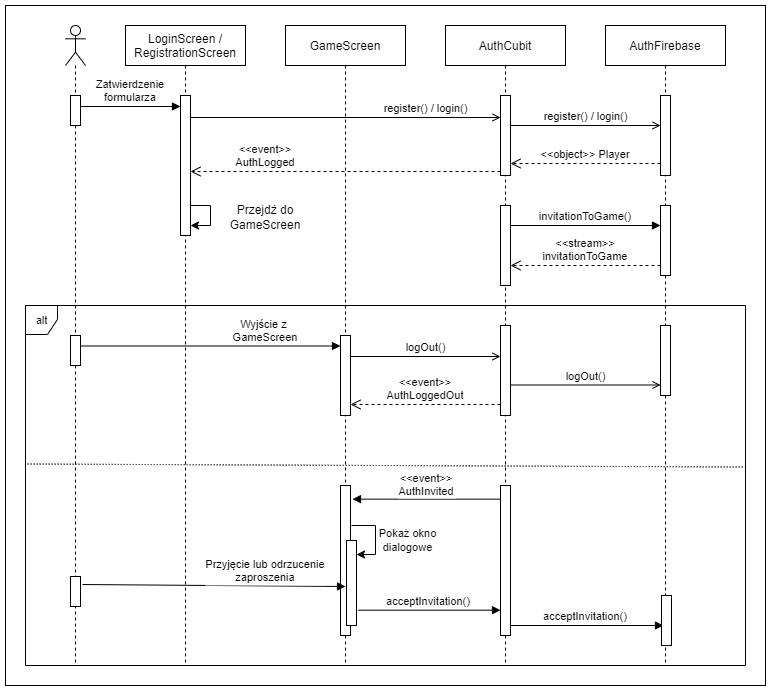
\includegraphics[width=16cm,height=12cm]{img/diagram-sekwencji-auth.png}
	\end{center}
	\caption{{\color{dgray}Diagram sekwencji obsługi konta użytkownika.}} 
	\label{AuthCubit}
\end{figure}

Powyższy diagram przedstawia interakcje pomiędzy warstwami, które są związane z klasą \emph{AuthCubit}. Klasa ta po stronie warstwy prezentacji komunikuje się z klasami \emph{RegistrationScreen}, \emph{LoginScreen} oraz \emph{GameScreen}. W przypadku rejestracji lub logowania klasa \emph{AuthCubit} jest pośrednikiem między warstwą prezentacji, a warstwą danych. Wywołuje asynchroniczą metodę \emph{login} z parametrami email oraz hasło, lub metodę \emph{register} (rozszerzona o dodatkowy parametr: nazwa użytkownika). Z warstwy prezentacji w odpowiedzi dostajemy obiekt \emph{Player}, który zawiera dwa atrybuty: ID gracza oraz jego nazwa. Następnie \emph{AuthCubit} przesyła strumieniem klasę stanu \emph{AuthLogged}, która zawiera otrzymany obiekt. \emph{LoginScreen} bądź \emph{RegistrationScreen} po otrzymaniu tego stanu, nawigują do strony \emph{GameScreen}, przekazując refernecję do \emph{AuthCubit} oraz parametry gracza. Ponadto po zalogowaniu / zarejestrowaniu użytkownika klasa \emph{AuthCubit} pobiera obiekt listenera z \emph{AuthFirebase}, za pomocą którego będzie nasłuchiwać pojawiające się zaproszenia innych użytkowników do rozgrywki. W przypadku interakcji \emph{GameScreen} z \emph{AuthCubit} występują dwa od siebie niezależne procesy. Pierwszy z nich polega na obsłudze wylogowania użytkownika. Natomiast drugi odpowiada za obsługę zaproszeń do gry. \emph{AuthCubit} po otrzymaniu komunikatu ze strumienia o zaproszeniu, emituję klasę stanu \emph{AuthInvited}, która zawiera nazwę zapraszającego i kod ID gry. W przypadku gdy gracz odmówi udziału, zostanie przekazana metoda \emph{acceptInvitation(false)}.

\begin{figure}[h!]
	\begin{center}
		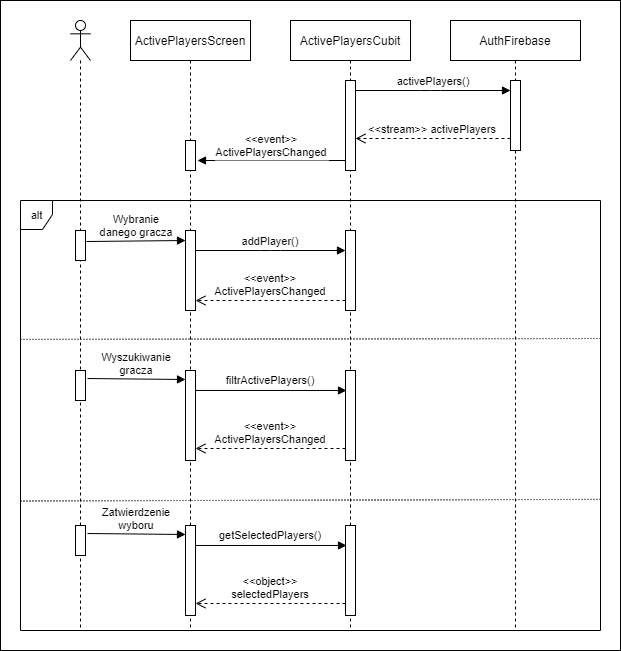
\includegraphics[width=14cm,height=12cm]{img/diagram-sekwencji-activePlayers.png}
	\end{center}
	\caption{{\color{dgray}Diagram sekwencji wyszukiwania aktywnych użytkowników.}} 
	\label{ActivePlayersCubit}
\end{figure}

Proces na rysunku 4.5 rozpoczyna się pobraniem strumienia z \emph{AuthFirebase}, dzięki któremu można otrzymywać aktualną listę aktywnych użytkowników w grze. Za każdym razem, gdy lista użytkowników ulegnie zmianie, będzie przekazywana do \emph{ActivePlayersScreen} klasa stanu \emph{ActivePlayersChanged}. Klasa ta zawiera w sobie aktualną listę aktywnych użytkowników, ale również zawiera listę dotychczas wybranych przez użytkownika graczy. Następnie występują trzy możliwe procesy, które odpowiadają działaniom użytkownika. W momencie, gdy gracz wybiera kogoś z listy, przekazywana jest nazwa wybranego gracza do \emph{ActivePlayersCubit} i zwracana jest zaktualizowana klasa stanu \emph{ActivePlayersChanged}. Użytkownik może również wyszukiwać gracza po nazwie. W tym przypadku za każdym razem zwracana jest klasa stanu, w której lista użytkowników jest odpowiednio przefiltrowana. Ostatnią możliwością jest zatwierdzenie wyboru. W takim przypadku do \emph{ActivePlayersScreen} jest przekazywana ostateczna lista wybranych graczy do zaproszenia. \vspace{4cm} \\

\begin{figure}[h!]
	\begin{center}
		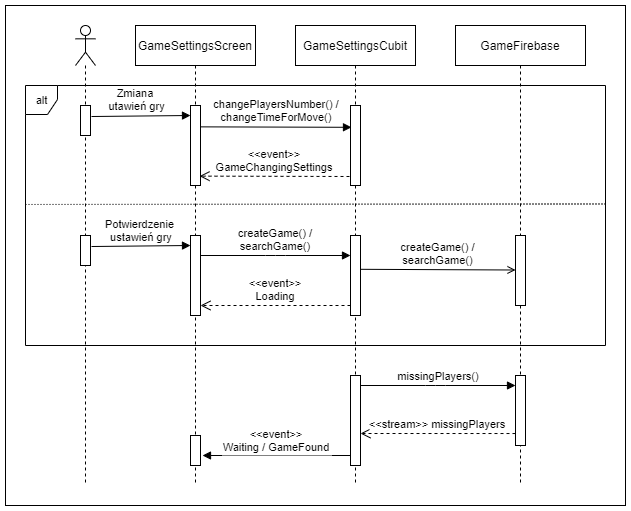
\includegraphics[width=14cm,height=13cm]{img/diagram-sekwencji-gameSettings.png}
	\end{center}
	\caption{{\color{dgray}Diagram sekwencji konfiguracji gry.}} 
	\label{GameSettingsCubit}
\end{figure} 

Dwa początkowe procesy ukazane na diagramie zależą od tego z jakimi parametrami została utworzona klasa \emph{GameSettingsCubit}. W przypadku, gdy gracz szuka gry do dołączenia może odpowiednio skonfigurować ustawienia gry, zmieniając liczbę graczy oraz czas przeznaczony na  wykonanie ruchu. Jeśli jednak gracz wybrał opcję stworzenia własnej gry z wybranymi graczami, może jedynie zmienić czas przeznaczony na ruch. Klasa stanu \emph{GameSettingsChanged} zawiera aktualnie wybrane ustawienia. Gdy użytkownik potwierdzi ustawienia za pośrednictwem \emph{GameSettingsCubit} w \emph{GameFirebase} jest wywoływana metoda \emph{createGame} (parametry: kod ID gracza, lista nazw zaproszonych graczy, czas przeznaczony na ruch w grze) lub metoda \emph{searchGame} (parametry: kod ID gracza, liczba graczy w grze, czas przeznaczony na ruch w grze). \emph{GameSettingsScreen} po otrzymaniu eventu \emph{Loading}, zastępuję dotychczasowy widok obracającym się kółeczkiem. W ostatnim procesie metoda \emph{missingPlayers} z parametrem ID gry, zwraca strumień, który powiadamia o dołączających graczach do gry. Klasa stanu \emph{Waiting} zawiera liczbę brakujących graczy do rozpoczęcia gry. Klasa \emph{GameFound} zawiera ID gry i wskazuje, że gra jest już gotowa do rozpoczęcia. W przypadku, gdy gracz przyjął zaproszenie do gry wykona się jedynie ostatni proces z pominięciem dwóch pierwszych, ponieważ gracz nie ma już wpływu na ustawienia gry. \\ \\ \\ \\ \\

\begin{figure}[h!]
	\begin{center}
		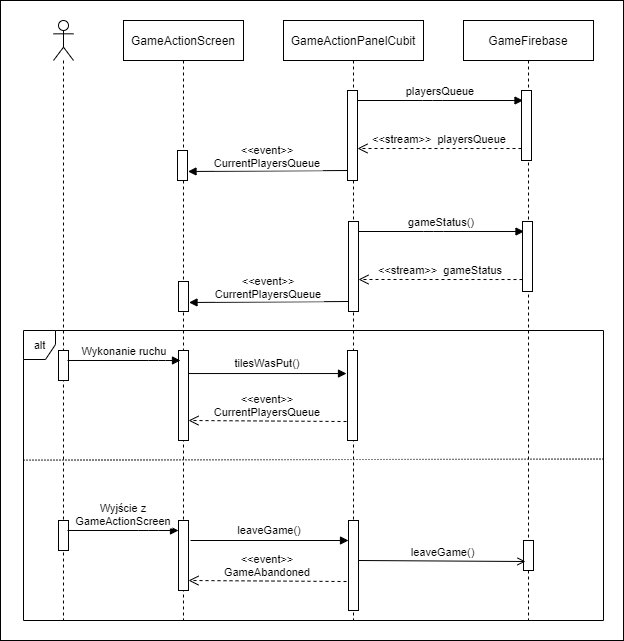
\includegraphics[width=14cm,height=13cm]{img/diagram-sekwencji-panel.png}
	\end{center}
	\caption{{\color{dgray}Diagram sekwencji panelu sterowania gry.}} 
	\label{GameActionPanelCubit}
\end{figure} 

Klasa \emph{GameActionPanelCubit} jest odpowiedzialna za zarządzanie stanem gry. Korzysta z dwóch strumieni danych. Strumień \emph{playersQueue} przekazuje aktualną listę uczestników gry, a \emph{gameStatus} wskazuje, jaki gracz ma obecnie prawo ruchu oraz czy pojawił się już zwycięzca gry. Informacje te są przekazywane do \emph{GameActionScreen}. Klasa stanu \emph{CurrentPlayersQueue} zawiera listę uczestników w grze oraz czas, który pozostał dla gracza mającego prawo ruchu. Kolejny proces przedstawia sytuację, gdy użytkownik wykonał wyłożenie kości. Wtedy informuje o tym \emph{GameActionPanelCubit}, które zeruje i przestaje odliczać czas jego ruchu. Ostatni proces dotyczy zdarzenia, gdy użytkownik zamierza opuścić grę przed jej zakończeniem. Cubit wywołuje metodę \emph{leaveGame} z parametrami: ID gracza oraz ID gry. \\ \\ \\ \\ \\ \\ \\ \\ \\ \\ \\

\begin{figure}[h!]
	\begin{center}
		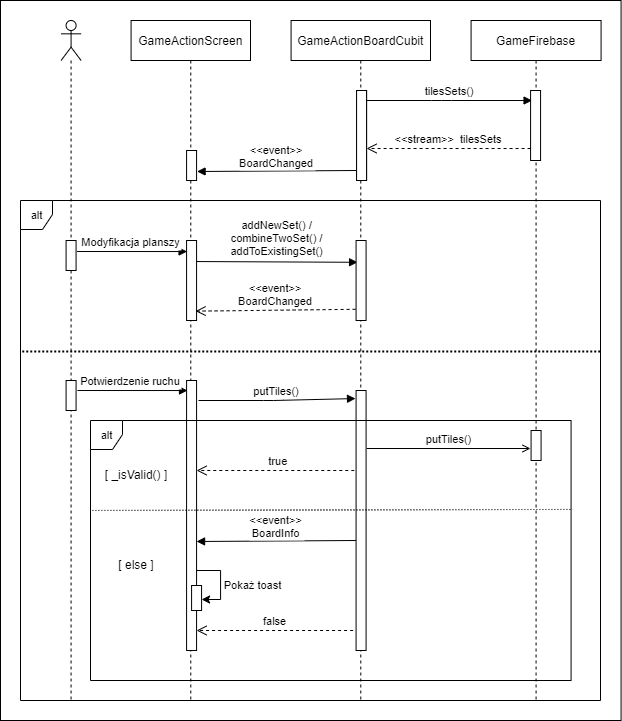
\includegraphics[width=14cm,height=13cm]{img/diagram-sekwencji-board.png}
	\end{center}
	\caption{{\color{dgray}Diagram sekwencji planszy rozgrywki.}} 
	\label{GameActionBoardCubit}
\end{figure} 

Klasa \emph{GameActionBoardCubit} jest odpowiedzialna za zarządzanie planszą gry. Pobiera strumień z \emph{GameFirebase}, który będzie przekazywał modyfikacje planszy przeprowadzone przez innych użytkowników. Klasa stanu \emph{BoardChanged} zawiera listę zbiorów kości. Następnie są obsługiwane dwa procesy dotyczące planszy. Proces pierwszy aktualizuje stan planszy za każdym razem, gdy gracz dokona modyfikacji pod warunkiem, że ma prawo ruchu. Modyfikacje mogą odbywać się trzema sposobami: \emph{addNewSet} dodanie kości do planszy tworzy nowy zbiór, \emph{combineTwoSet} dodanie kości łączy dwa zbiory, \emph{addToExistingSet} kość jest dodwana do istniejącego zbioru. Drugi proces następuje, gdy gracz chce zatwierdzić swoje zmiany przeprowadzone na planszy. W takim przypadku \emph{GameActionBoardCubit} przeprowadza walidację stanu planszy. Metoda \emph{\_isValid} wskazuje, czy otrzymany zbiór kości jest zgodny z zasadami gry. Jeśli tak to zostanie wywołana funkcja dodania kości po stronie \emph{GameFirebase}, w przeciwnym wypadku zostanie wyświetlone powiadomie o tym, że plansza nie jest ułożona w poprawny sposób. W momencie, gdy czas gracza minął, a ten nie zdążył wyłożyć kości o poprawnej konfiguracji, plansza wraca do stanu sprzed modyfikacji ze strony danego gracza. \\ \\ \\ \\ \\ \\

\begin{figure}[h!]
	\begin{center}
		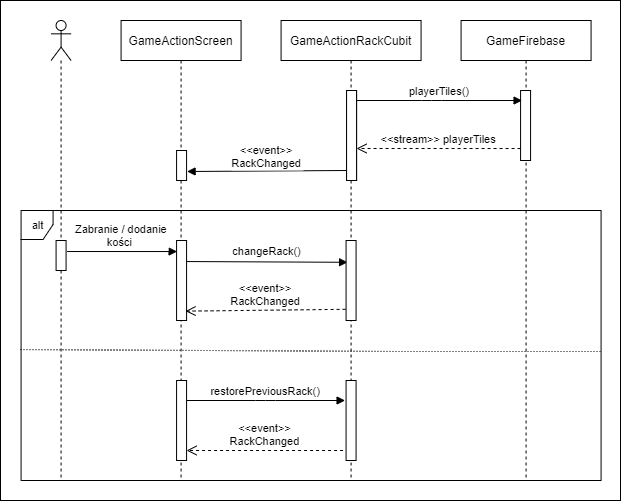
\includegraphics[width=13cm,height=10cm]{img/diagram-sekwencji-rack.png}
	\end{center}
	\caption{{\color{dgray}Diagram sekwencji zestawu kości gracza.}} 
	\label{GameActionRackCubit}
\end{figure} 

Klasa \emph{GameActionRackCubit} jest odpowiedzialna za zarządzanie zbiorem kości gracza. Pobiera strumień z \emph{GameFirebase}, który będzie przekazywał zmiany zachodzące w zbiorze kości (w przypadku braku wyłożenia gracz będzie otrzymywał kość z banku). Klasa stanu \emph{RackChanged} zawiera listę kości. W momencie, gdy gracz wykłada kości na plansze, albo z powrotem wkłada (może wziąć z planszy tylko swoje kości), klasa \emph{GameActionRackCubit} jest informowana i aktualizuje listę kości gracza. W przypadku gdy czas gracza minął jest wykonywana funkcja \emph{restorePreviousRack}, poprzez którą zmiany dokonane przez gracza w czasie swojego ruchu są anulowane. \emph{GameActionRackCubit} zapamiętuje stan zestawów kości w momencie rozpoczęcia ruchu przez gracza.
